% mnras_template.tex
%
% LaTeX template for creating an MNRAS paper
%
% v3.0 released 14 May 2015
% (version numbers match those of mnras.cls)
%
% Copyright (C) Royal Astronomical Society 2015
% Authors:
% Keith T. Smith (Royal Astronomical Society)

% Change log
%
% v3.0 May 2015
%    Renamed to match the new package name
%    Version number matches mnras.cls
%    A few minor tweaks to wording
% v1.0 September 2013
%    Beta testing only - never publicly released
%    First version: a simple (ish) template for creating an MNRAS paper

%%%%%%%%%%%%%%%%%%%%%%%%%%%%%%%%%%%%%%%%%%%%%%%%%%
% Basic setup. Most papers should leave these options alone.
\documentclass[fleqn,usenatbib]{mnras}

% MNRAS is set in Times font. If you don't have this installed (most LaTeX
% installations will be fine) or prefer the old Computer Modern fonts, comment
% out the following line
\usepackage{newtxtext,newtxmath}
% Depending on your LaTeX fonts installation, you might get better results with one of these:
%\usepackage{mathptmx}
%\usepackage{txfonts}

% Use vector fonts, so it zooms properly in on-screen viewing software
% Don't change these lines unless you know what you are doing
\usepackage[T1]{fontenc}
\usepackage{ae,aecompl}


%%%%% AUTHORS - PLACE YOUR OWN PACKAGES HERE %%%%%

% Only include extra packages if you really need them. Common packages are:
\usepackage{graphicx} % Including figure files
\usepackage{amsmath} % Advanced maths commands
\usepackage{amssymb} % Extra maths symbols
\usepackage{xcolor} % Colour text for draft

%%%%%%%%%%%%%%%%%%%%%%%%%%%%%%%%%%%%%%%%%%%%%%%%%%

%%%%% AUTHORS - PLACE YOUR OWN COMMANDS HERE %%%%%

% Please keep new commands to a minimum, and use \newcommand not \def to avoid
% overwriting existing commands. Example:
%\newcommand{\pcm}{\,cm$^{-2}$} % per cm-squared

% Use bold font for vectors
\let\vec\mathbf

%%%%%%%%%%%%%%%%%%%%%%%%%%%%%%%%%%%%%%%%%%%%%%%%%%

%%%%%%%%%%%%%%%%%%% TITLE PAGE %%%%%%%%%%%%%%%%%%%

% Title of the paper, and the short title which is used in the headers.
% Keep the title short and informative.
\title[Large Stokes number multigrain]{Large Stokes number multigrain: A
smoothed particle hydrodynamics algorithm for large dust grains}

% The list of authors, and the short list which is used in the headers.
% If you need two or more lines of authors, add an extra line using \newauthor
\author[Mentiplay, Price, Pinte, \& Laibe]{%
   \parbox{\textwidth}{%
      Daniel Mentiplay\(^{1}\)\thanks{daniel.mentiplay@monash.edu},
      Daniel J. Price\(^{1}\),
      Christophe Pinte\(^{1,2}\),
      Guillaume Laibe\(^{3}\)}\\
   \(^{1}\)Monash Centre for Astrophysics (MoCA) and School of Physics and
   Astronomy, Monash University, Clayton Vic 3800, Australia \\
   \(^{3}\)Lyon, France \\
   \(^{2}\)Univ. Grenoble Alpes, CNRS, IPAG, F-38000 Grenoble, France}

% These dates will be filled out by the publisher
\date{Accepted XXX. Received YYY; in original form ZZZ}

% Enter the current year, for the copyright statements etc.
\pubyear{2020}

% Don't change these lines
\begin{document}
\label{firstpage}
\pagerange{\pageref{firstpage}--\pageref{lastpage}}
\maketitle

% Abstract of the paper
\begin{abstract}
   We present a new method for simulating the dynamics of a mixture of gas and
   multiple species of large Stokes number dust grains, typical of evolved
   protoplanetary discs and debris discs. The method improves upon earlier
   methods, in which only a single grain size could be represented, by capturing
   the differential backreaction of multiple dust species on the gas. This
   effect is greater for large dust-to-gas ratios that may be expected in the
   later stages of the protoplanetary disc life.
\end{abstract}

% Select between one and six entries from the list of approved keywords.
% Don't make up new ones.
\begin{keywords}
hydrodynamics -- methods: numerical -- protoplanetary discs
\end{keywords}

%%%%%%%%%%%%%%%%%%%%%%%%%%%%%%%%%%%%%%%%%%%%%%%%%%

%%%%%%%%%%%%%%%%% BODY OF PAPER %%%%%%%%%%%%%%%%%%

\section{Introduction}

\textcolor{red}{
\begin{itemize}
   \item Dust-gas modeling in astrophysical fluids.
   \item Single grain size vs multiple dust species.
   \item \citet{Haworth2016PASA...33...53H}---grand challenges in protoplanetary disc
      modeling.
   \item Applications: protoplanetary discs, debris discs.
   \item Phantom dust methods---\citet{Price2018PASA...35...31P}.
   \item Phantom 1-fluid multigrain---\citet{Hutchison2018MNRAS.476.2186H}.
\end{itemize}
}

\section{Methods}

\subsection{Continuum equations for multiple dust species}

We consider a mixture of gas, indexed by \(g\), and \(N\) dust species, indexed
by \(d_i\). We neglect the finite size of the dust particles, and thus set the
gas volume fraction to unity. We represent each dust species as a continuous
fluid with a fixed size, \(s_i\), and intrinsic density, \(\varrho_{m_i}\).
Then, the equations of conservation of mass for the mixture is given by
%
\begin{align}
   \label{eqn:conserve-mass}
   \frac{\partial \rho_g}{\partial t} + \nabla \cdot (\rho_g \vec{v}_g) &= 0, \\
   \frac{\partial \rho_{d_i}}{\partial t} + \nabla \cdot (\rho_{d_i} \vec{v}_{d_i}) &= 0,
\end{align}
%
for each \(i\) in 1 to \(N\), where \(\rho_j\) and \(\vec{v}_j\) are the density
and velocity of the fluids.

We assume the fluids are inviscid, that the dust is pressureless, and that each
dust species is homogeneous, i.e.\ has the same mass, size, and intrinsic
density. The equations of conservation of momentum for the mixture are given by
%
\begin{align}
   \rho_g \frac{\mathrm{d} \vec{v}_g}{dt}
      &= - \nabla P + \rho_g \vec{f} + \sum_i K_i \left(\vec{v}_{d_i}
         - \vec{v}_{g}\right), \\
   \rho_{d_i} \frac{\mathrm{d} \vec{v}_{d_i}}{dt}
      &= \rho_{d_i} \vec{f} - K_i \left(\vec{v}_{d_i} - \vec{v}_{g}\right),
\end{align}
%
where \(P\) is the gas pressure, \(\vec{f}\) is any body forces acting on the
fluids, and \(K_i\) is the drag coefficient between the gas and a particular
dust species, \(i\). Note that each dust fluid has one gas drag interaction
term, whereas the gas momentum equation has a sum of interactions over each dust
species. Also note that the dust has no pressure gradient force term. In
general, the drag coefficient could be a complicated expression. We assume that
the drag coefficient is linear with respect to the differential velocity,
\(\Delta \vec{v}_i = \vec{v}_{d_i} - \vec{v}_g \).

The gas and dust exchange momentum via drag which leads to frictional heating.
Under the assumption that the gas and dust grains are at the same temperature,
the evolution of gas internal energy is given by
%
\begin{align}
   \label{eqn:conserve-energy}
   \rho_g \frac{\mathrm{d} u_g}{\mathrm{d} t} =
      - P \nabla \cdot \vec{v}_g + \rho_g \sum_i K_i (\vec{v}_g - \vec{v}_{d_i})^2.
\end{align}
%
We neglect the dust fluid internal energy under the assumption that the dust and
gas are at the same temperature.

Equations~\ref{eqn:conserve-mass}--\ref{eqn:conserve-energy} are \(2N + 3\)
equations describing the evolution of a mixture of gas and \(N\) dust species.
We discuss discretising these equations with smoothed particle hydrodynamics in
Section~\ref{subsec:sph}.

\subsection{Drag timescale}

\textcolor{red}{
\begin{itemize}
   \item Discuss large grains vs small grains and strong vs weak coupling in the
      context of Stokes number, and terminal velocity approximation.
\end{itemize}
}

\subsubsection{Stopping time}

Dust and gas interact via a drag force. This drag force has a characteristic
time scale, known as the stopping time. The stopping time relates to the drag
coefficient, which depends on quantities such as the gas temperature and
density, and on the physical characteristics of the dust grains. For a single
dust species, the stopping time, \(t_s\), is given by
%
\begin{align}
   \label{eqn:stopping-time}
   t_s = \frac{\rho_g \rho_d}{K (\rho_g + \rho_d)},
\end{align}
%
where \(K\) is the drag coefficient for the single species. We assume spherical
grains of size \(s\) with a uniform material density, \(\varrho_m\). In the
linear Epstein regime \citep{Epstein1924PhRv...23..710E} the drag coefficient
\(K\) is
%
\begin{align}
   \label{eqn:drag-coefficient}
   K = \frac{\rho_g \rho_d}{\varrho_m s} \sqrt{\frac{8}{\pi\gamma}} c_s.
\end{align}
%
For convenience, we define an effective material density,
\(\varrho_{\mathrm{eff}}\), given by \(\varrho_{\mathrm{eff}} = \varrho_m
\sqrt{\pi\gamma/8}\).

As discussed in \citet{Hutchison2018MNRAS.476.2186H}, a straightforward
generalisation of the stopping time for multiple dust species is not available.
Each dust species is separately coupled to the gas by the drag force. However,
the dust species are indirectly coupled to each other via backreaction, as
required conservation of momentum. Considering the multiple dust species case,
the drag coefficient, \(K_i\), is now
%
\begin{align}
   K_i = \frac{\rho_g \rho_{d_i} c_s}{\varrho_{\mathrm{eff}} s_i}.
\end{align}
%
We define \(\rho = \rho_g + \sum_i \rho_{d_i}\) as the total density of the gas
and all dust species, and the weighted sum \(s_{\mathrm{eff}} = \sum_i
\rho_{d_i} s_i / \sum_i \rho_{d_i}\) as an effective grain size for the mixture.
Then we can define an effective stopping time for the dust mixture as
%
\begin{align}
   \label{eqn:effective-stopping-time}
   T_s = \frac{\varrho_{\mathrm{eff}} s_{\mathrm{eff}}}{\rho c_s}.
\end{align}
%
By combining Equations~\ref{eqn:stopping-time}~\&~\ref{eqn:drag-coefficient} we
can see the expression for the multigrain effective stopping time is analogous
to the single dust species case.

\subsubsection{Stokes number}

The Stokes number, \(\mathrm{St}\), is a dimensionless stopping time defined as
the stopping time in units of a typical flow time. For protoplanetary discs, the
typical flow time is the Keplerian orbital time, \(1/\Omega_K\), so that the
Stokes number is \(\mathrm{St} = t_s \Omega_K\). Note that the Stokes number
depends on the gas disc properties, via the density and temperature, the dust
disc density, the dust grain properties, i.e. size and material density, and the
stellar mass and orbital distance. The disc surface density, \(\Sigma\), and
disc scale height, \(H\), are related to the density, sound speed, and Keplerian
orbital time by \(\rho = \Sigma / H\) and \(\Omega_K = c_s / H\). Using these
relations we can show that the Stokes number in the midplane of a protoplanetary
disc is given by
%
\begin{align}
   \mathrm{St} = \frac{\varrho_{\mathrm{eff}} s}{\Sigma}.
\end{align}
%
In using \(\rho = \Sigma / H\) and \(\Omega_K = c_s / H\) to derived the above
expression we are assuming that the gas mass dominates over the dust mass, i.e.
that the dust fraction is low. Otherwise we must consider that the scale height
varies between the gas disc and the dust sub-discs.

Considering the multiple dust species case, we can define an effective midplane
Stokes number for the mixture using the effective stopping time
(Equation~\ref{eqn:effective-stopping-time}) as \(\mathrm{St}_{\mathrm{eff}} =
\varrho_{\mathrm{eff}} s_{\mathrm{eff}} / \Sigma \). An alternative is to define
a per species midplane Stokes number in analogy with the single grain size case:
%
\begin{align}
   \mathrm{St}_i = \frac{\varrho_{\mathrm{eff}} s_i}
      {\Sigma_g \left(1 + \sum_i \varepsilon_i \right)},
\end{align}
%
where \(\Sigma_g\) is the gas surface density and \(\varepsilon_i\) is the
dust-to-gas ratio for each dust species. Again we see the combination of grain
properties, size and material density, and the disc surface density fixing the
Stokes number. Given that we assume the material density is the same for all
species, we see that the grain size of the species, for any fixed location in
the disc, gives the variation in Stokes number between species.

\subsection{SPH with multiple dust species}%
\label{subsec:sph}

\textcolor{red}{
\begin{itemize}
   \item For ``two-fluid'' see \citet{Laibe2012MNRAS.420.2345L}, Section 2.2.
\end{itemize}
}

\subsection{Time stepping}

\textcolor{red}{
\begin{itemize}
   \item Explicit time stepping.
   \item Drag timescale limits calculation to \(\mathrm{St} \gtrsim 1\).
\end{itemize}
}

\section{Numerical tests}

\subsection{Dusty-box}

\begin{figure*}
   \begin{center}
      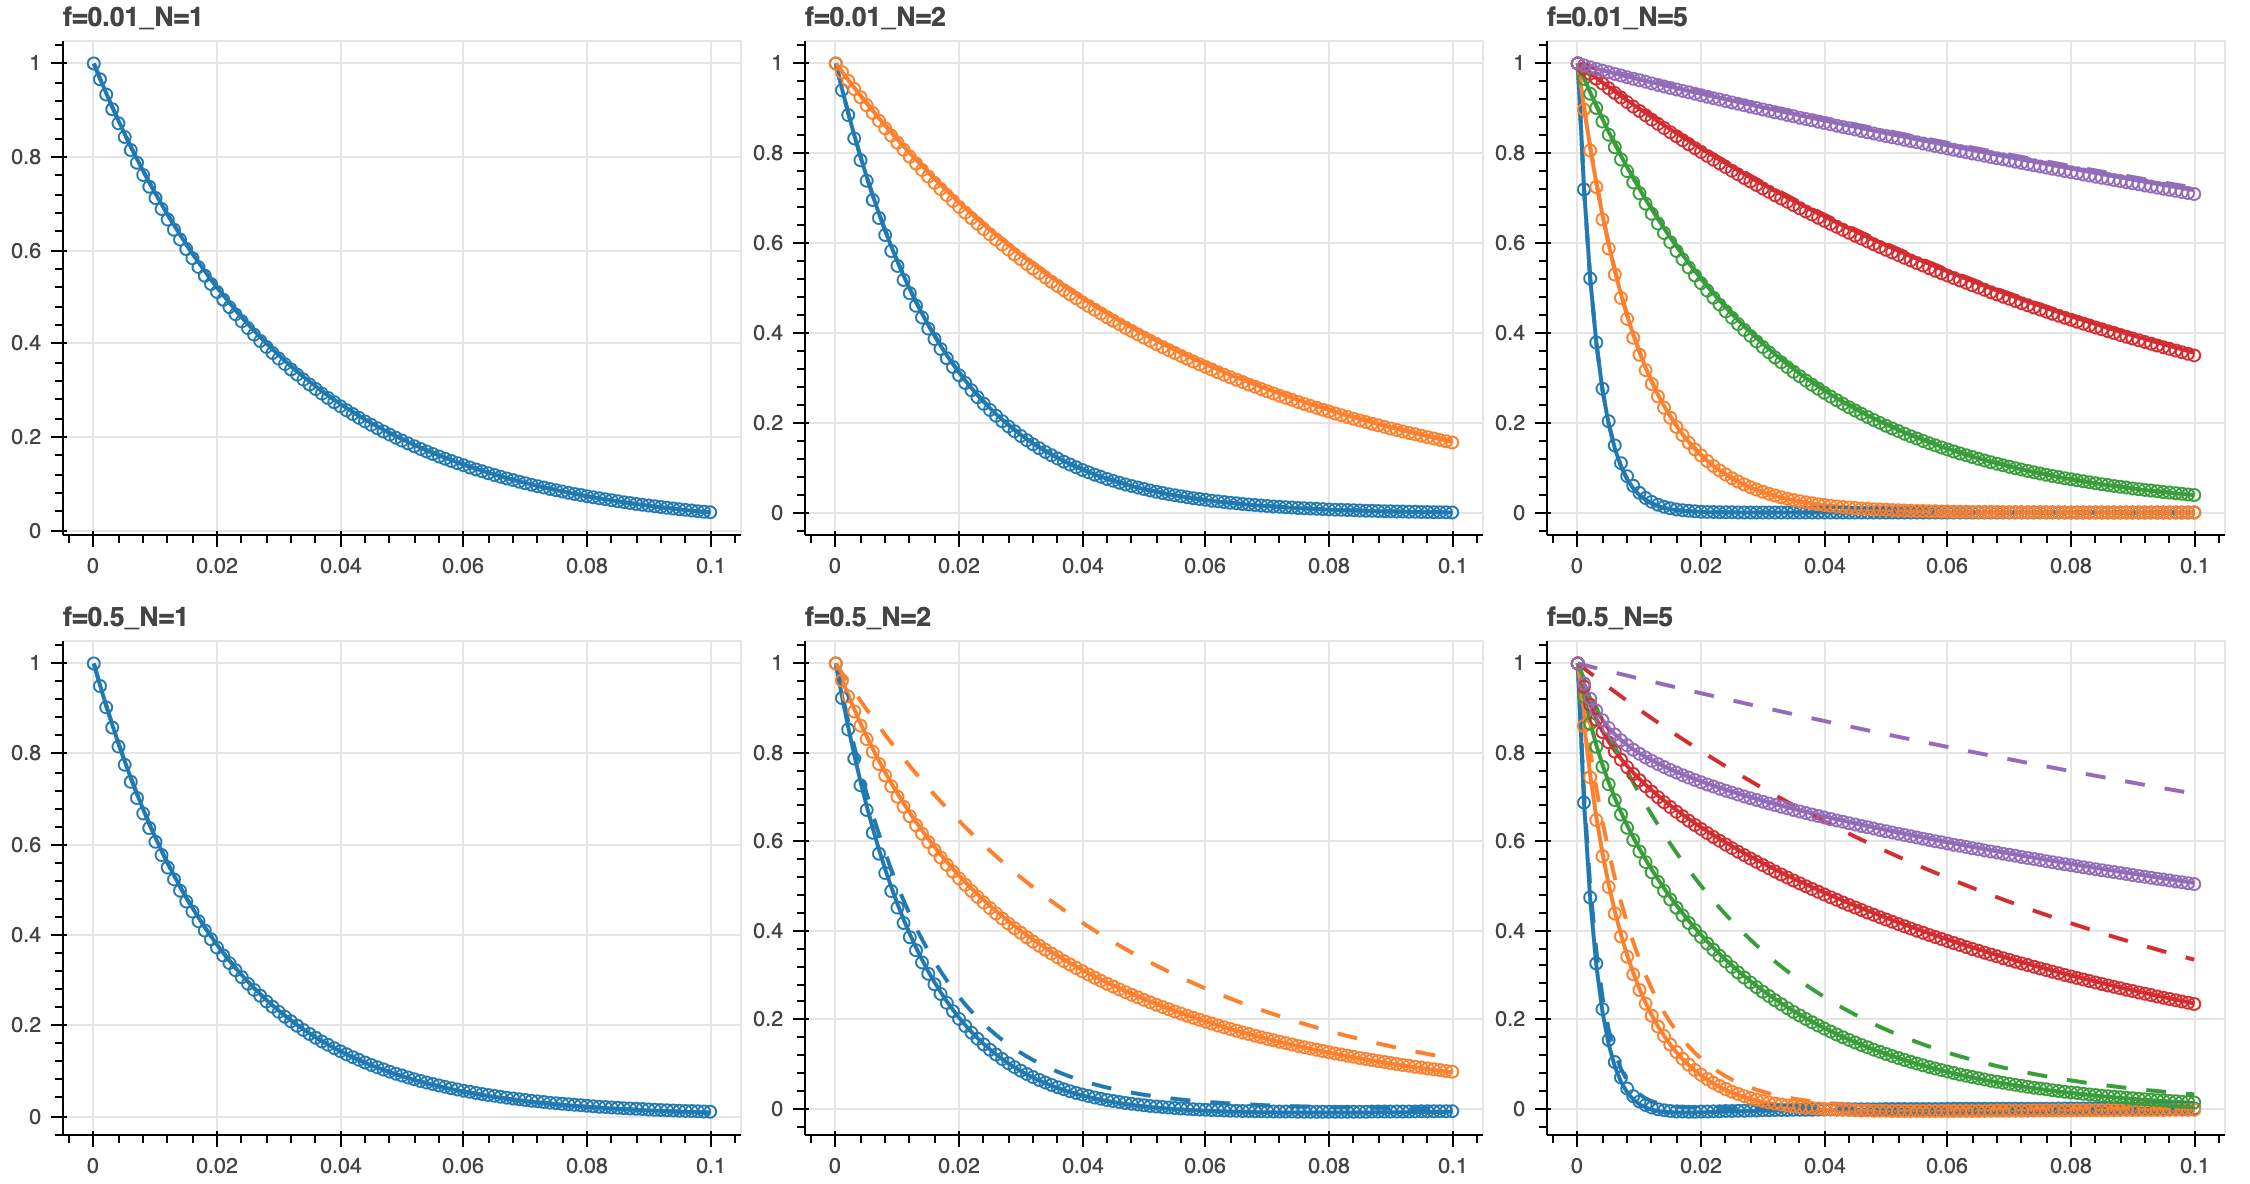
\includegraphics[width=\textwidth]{figs/dustybox.png}
      \caption{Dusty-box numerical test showing the differential velocity
         between the dust and gas. The total dust-to-gas ratio is 0.01 (top row)
         and 0.5 (bottom row). From left to right: the number of dust species is
         1, 2, 5. The open circles represent the results from the Phantom
         simulation. The solid and dashed lines represent the analytical
         solution with and without taking back reaction into account,
         respectively.\label{fig:dustybox}}
   \end{center}
\end{figure*}

We performed the multigrain version of the dusty-box test described in
\citet{Laibe2011MNRAS.418.1491L}. The dusty-box involves setting up a periodic
box of uniform density gas and dust with an initial differential velocity
between the gas and dust. In this test the equation of motion simplifies to
%
\begin{align}
   \frac{\partial \Delta \vec{V}}{\partial t} = - \Omega_n \Delta \vec{V},
\end{align}
%
where \(\Delta \vec{V}\) is the differential velocity vector, i.e.
\(\vec{v}_{d_i} - \vec{v}_g\) for each \(i\), and \(\Omega_n\) is the drag
matrix given in Eq.~64 of \citet{Laibe2014MNRAS.444.1940L}. Dusty-box is a test
of the exchange of momentum between gas and dust species via the drag force. The
original dusty-box test was for a single grain size. We ran the multigrain
version described in \citet{Laibe2014MNRAS.444.1940L} in the linear Epstein drag
regime \citep{Epstein1924PhRv...23..710E}. We chose the physical Epstein drag
prescription in Phantom.

\begin{table}
   \centering
   \begin{tabular}{ccc}
      \hline
      \hline
      Species & Grain size [cm] \\
      \hline
      \hline
      One dust species \\
      1 & 1.0 \\
      \hline
      Two dust species \\
      1 & 0.562 \\
      2 & 1.78 \\
      \hline
      Five dust species \\
      1 & 0.1 \\
      2 & 0.316 \\
      3 & 1.0 \\
      4 & 3.16 \\
      5 & 10.0 \\
      \hline
      \hline
   \end{tabular}
   \caption{Grain sizes for dusty box test.}
   \label{tab:dustybox}
\end{table}

We performed six tests in two sets of three. The first set had a total
dust-to-gas ratio of 0.01, and the second set 0.5. The tests within each set had
1, 2, and 5 dust species, respectively, with grain sizes given in
Table~\ref{tab:dustybox}. Each test had equal mass in each grain size bin. The
gas is initially motionless, and each dust species has uniform velocity in the
positive x-direction.

For each test problem, we set up each of the gas and dust fluids on a
close-packed lattice, such that there were 32 gas particles in the direction of
motion, and, for each dust species, 16 dust particles. We set the gas density to
\(10^{-13}\)~g~cm\({}^{-3}\), with dust density varying per test problem. We set
the dust grain density to \(0.5 \times 10^{-14}\)~g~cm\({}^{-3}\).

Figure~\ref{fig:dustybox} shows the time evolution of the mean velocity
differential between the gas and each dust species, compared with analytical
solutions. The dashed lines represent the analytical solution without
backreaction from the dust on the gas. The solid lines represent the analytical
solution including backreaction. For low dust-to-gas ratio (0.01) both
analytical solutions give the same decay of differential velocity, with which
the Phantom simulation agrees. For a larger dust-to-gas ratio (0.5) the
analytical solutions diverge, and the Phantom simulation data follows the
backreaction-inclusive solution. For large dust-to-gas ratio we see that the
smaller grains (0.1 cm and 0.316 cm) rapidly slow and the differential velocity
reverses sign. I.e. the small grains slow to the gas velocity; then, as the
larger grains speed up the gas via drag, the gas drags the small grains along
with it. This shows that the behaviour of multiple dust species for large
dust-to-gas ratios requires taking back reaction into consideration to capture
the physics of dust drag accurately
\citep{Gonzalez2017MNRAS.467.1984G,Dipierro2018MNRAS.479.4187D}.

\subsection{Dusty-wave}

\begin{figure*}
   \begin{center}
      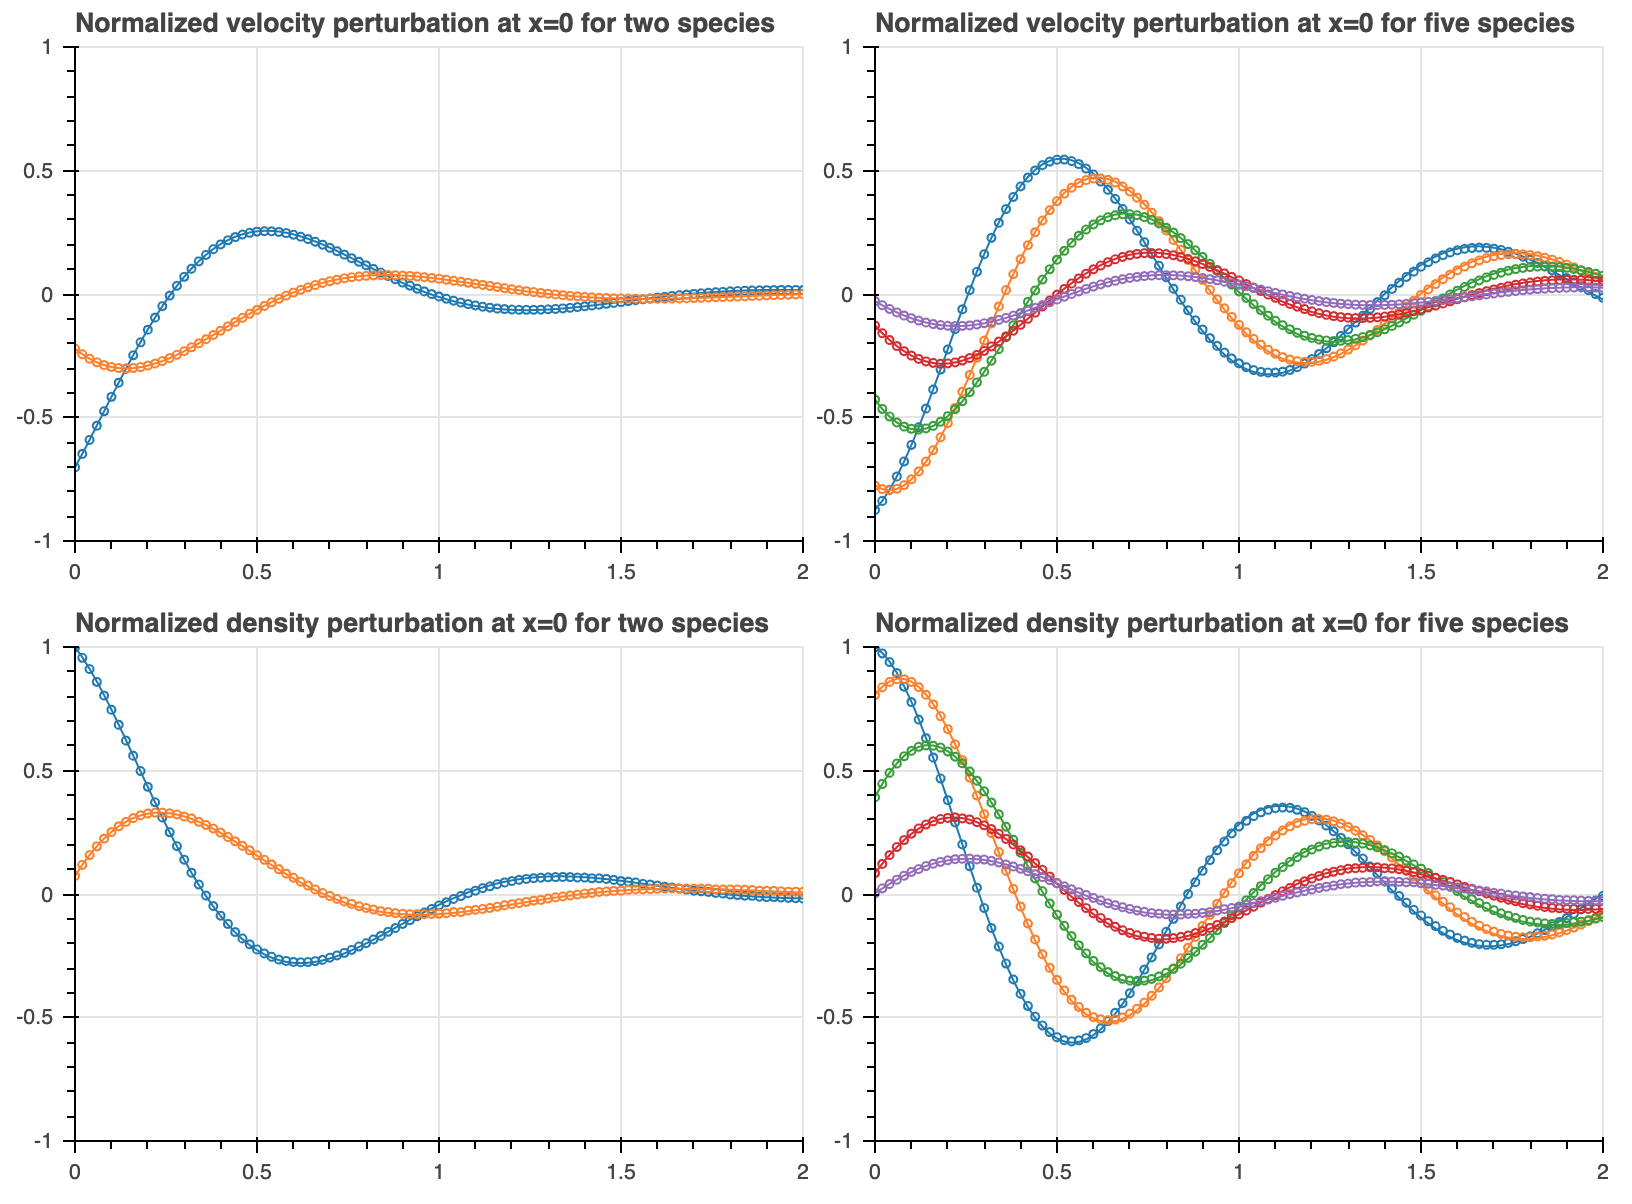
\includegraphics[width=\textwidth]{figs/dustywave.png}
      \caption{Dusty-wave numerical test showing the normalised velocity (top)
         and density (bottom) perturbation at \(x = 0\), for gas with one dust
         species (left) and gas with four dust species (right). The open circles
         represent the Phantom simulation, and the solid line represents the
         analytical solution from
         \citet{Benitez-Llambay2019ApJS..241...25B}.\label{fig:dustywave}}
   \end{center}
\end{figure*}

We performed the multigrain version of the dusty-wave test described in
\citet{Laibe2011MNRAS.418.1491L}. This is a test of the dust-gas drag coupling
in the context of a damped sound wave. The dust is a pressureless fluid and
cannot support sound waves. However, the gas can support sounds waves and drags
the dust. This leads to damping of the wave.

Considering small perturbations around an equilibrium state, \(\rho_j = \rho_j^0
+ \delta \rho_j\), and \(v_j = \delta v_j\), where \(j\) is \(g\) for the gas
species, and \(d_i\) for each of the dust species, the linearised equations of
motion for this system are
%
\begin{align}
   \frac{\partial \delta \rho_g}{\partial t}
      + \rho_g^0 \frac{\partial \delta v_g}{\partial x} &= 0, \\
   \frac{\partial \delta \rho_{d_i}}{\partial t}
      + \rho_{d_i}^0 \frac{\partial \delta v_{d_i}}{\partial x} &= 0, \\
   \rho_g^0 \frac{\partial \delta v_g}{\partial t}
      &= \sum_i K_i \left(\delta v_{d_i} - \delta v_g \right)
         + c_s^2 \frac{\partial \delta \rho_g}{\partial x}, \\
   \rho_{d_i}^0 \frac{\partial \delta v_{d_i}}{\partial t}
      &= - K_i \left(\delta v_{d_i} - \delta v_{g}\right).
\end{align}
%
For the particular setup we followed \citet{Benitez-Llambay2019ApJS..241...25B}.
They derive solutions for the above equations as a dispersion relation (their
equation 45) and associated set of eigenfunctions (their equations 46--48).
Following \citet{Benitez-Llambay2019ApJS..241...25B}, we set the initial
condition to constant density and zero velocity, with perturbations of the form
%
\begin{align}
   \delta f = A \left[\mathrm{Re} \left(\delta \hat{f} \right) \cos(kx)
      - \mathrm{Im} \left(\delta \hat{f} \right) \sin(kx) \right],
\end{align}
%
where each perturbation can be written \(\delta f = \delta \hat{f} e^{ikx -
i\omega t}\). We set the sound speed \(c_s = 1\), and the wave amplitude \(A\)
to \(10^{-4} c_s\) and \(10^{-4} \rho_g^0\) for the velocity and density
perturbations, respectively.

We performed two tests: (1) with gas and a single dust species, and (2) with gas
and four dust species. We set the background density, drag coefficients, and
initial perturbations from Table 2 in
\citet{Benitez-Llambay2019ApJS..241...25B}. We chose a periodic box of unit
length, with 128 particles in the wave direction for each species. We use
constant drag, \(K_i\), for each dust species, with \(K_i = \rho_{d_i} /
t_{s_i}\), and \(\rho_{d_i}\) and \(t_{s_i}\) from Table 2.

Figure~\ref{fig:dustywave} shows the time evolution of the normalised velocity
and density perturbations at a particular location within the domain (\(x=0\)).
The solid lines represent the analytical solution from
\citet{Benitez-Llambay2019ApJS..241...25B} and the open circles represent the
numerical solution from Phantom. We first note that the numerical solution
accurately reproduces the analytical solution. In all cases we see the wave
damping effect.

\subsection{Dusty-shock}

\textcolor{red}{
See \citet{Laibe2012MNRAS.420.2345L}, \citet{Lehmann2018MNRAS.476.3185L}.
}


\section{Applications}

\subsection{Radial drift}

\textcolor{red}{
See example in \citet{Dipierro2018MNRAS.479.4187D}.
}

\subsection{Dust settling}

\textcolor{red}{
See Section~4.3 in \citet{Hutchison2018MNRAS.476.2186H}.
}

\subsection{Circumbinary disc}

\textcolor{red}{
Do a comparison between multiple single grain calculations vs one multigrain
calculation focussing on dust trapping in a circumbinary disc. For example, in
HD~142527. The figure would show a phase difference between the dust (or gas)
distribution comparing the single-grain vs multigrain calculation.
}

\section{Discussion}

\textcolor{red}{
\begin{itemize}
   \item Time step constraint via Stokes number. I.e.\ only appropriate for
      large grains.
   \item Memory constraint: extra set of particles per dust species requires
      position, velocity, etc.\ unlike the mixture method.
\end{itemize}
}

\section{Conclusions}

\textcolor{red}{
\begin{itemize}
   \item Implemented SPH numerical scheme for multiple dust species represented
      by separate sets of SPH particles, appropriate for large Stokes number
      regime.
   \item Demonstrated that the method is accurate by testing on known problems.
   \item Applied the method to simulate physical processes in protoplanetary
      discs.
\end{itemize}
}

\section*{Acknowledgements}


%%%%%%%%%%%%%%%%%%%%%%%%%%%%%%%%%%%%%%%%%%%%%%%%%%

%%%%%%%%%%%%%%%%%%%% REFERENCES %%%%%%%%%%%%%%%%%%

% The best way to enter references is to use BibTeX:

\bibliographystyle{mnras}
\bibliography{multigrain-paper}


%%%%%%%%%%%%%%%%%%%%%%%%%%%%%%%%%%%%%%%%%%%%%%%%%%

%%%%%%%%%%%%%%%%% APPENDICES %%%%%%%%%%%%%%%%%%%%%

% \appendix

% \section{Some extra material}


%%%%%%%%%%%%%%%%%%%%%%%%%%%%%%%%%%%%%%%%%%%%%%%%%%


% Don't change these lines
\bsp % typesetting comment
\label{lastpage}
\end{document}
% End of mnras_template.tex
